
\subsection{Cross Validation\index{Cross Validation}}
\label{sec:cross:validation}

The goal of cross validation, and the larger framework of validation, is to estimate the performance of a machine learning model.

A model $\hat{f}(x | \theta)$ takes as input a data point $x$ and outputs a prediction for that data point given a set of tunable parameters $\theta$. The parameters are tuned through a training process using a training set, $\mathcal{T}$, for which the true output is known. This results in a model whose parameters are tuned to perform as good as possible on new, unseen, data.

The training error, $\overline{err}_{\mathcal{T}}$, for a model is defined as
\begin{equation}
\overline{err}_{\mathcal{T}} = \frac{1}{N_t}\sum_{n=1}^{N_t}L(y_n, \hat{f}(x_n))
\label{eq:train.err}
\end{equation}
where $N_t$ is the number of events used for training, $L$ is a chosen loss function, $\hat{f}$ is our model, and $x_n$ and $y_n$ are points in our training set.

The training error, in general, is a poor estimator of the performance of the model on new, unseen data. It is generally a decreasing function of the number of training iterations and unless the method is simple, i.e. has few tunable parameters, it can start to adapt to the noise in the training data. When this happens the training error continues to go down but the general performance, the error on data outside of the training set, starts increasing. This effect is called overfitting.

The test error, or prediction error, is defined as the expected error when the model is applied to new, unseed data.
\begin{equation}
Err_{\mathcal{T}} = E\left[L(Y,\hat{f}(X)) | \mathcal{T} \right]
\end{equation}
using the same notation as Eq~\ref{eq:train.err} and where $(X, Y)$ are two random variables drawn from the joint probability distribution. Here the model, $\hat{f}$, is trained using the training set, $\mathcal{T}$, and the error is evaluated over all possible inputs in the input space.

A related measure, the expected prediction error, additionally averages over all possible training sets
\begin{equation}
Err = E\left[L(Y, \hat{f}(X))\right] = E\left[Err_{\mathcal{T}}\right]
\end{equation}

This notation is inspired by \cite{Hastie01a}. To understand, and to more easily remember, what each quantity signifies one can consider whether it considers concrete data or random variables. The training error is defined for events in the training set and thus uses a minuscule initial letter. The prediction error is defined over the complete input space and uses random variables in the definition thus having a capital letter.
The subscript signifies what data was used to train the model.

The simplest way to reliably estimate $Err_{\mathcal{T}}$ is to to partition the initial data set into two parts and use one part for training and one part for testing. In the case where access to data is unlimited this method yields an optimal estimate.

However, often access to data is limited; For example in physics where the cost of generating Monte Carlo samples can be prohibitive, or in medical surveys where the number of respondents is limited. This means a choice has to be made, how much data should be used for training, and how much for evaluating the performance?

As a larger fraction of events are used for training, the performance of the final model increases due to better tuned parameters. However, our estimation of that performance becomes increasingly uncertain due to the limited size of the test set.

One way to reap the benefits of a large training set and large test set is to use cross validation. This discussion will focus on one technique in particular: K-folds.

In k-folds cross validation, initially introduced in \cite{Geisser75}, a data set is split into equal sized partitions, or folds. A model is then trained using one fold as test set and the concatenation of the remaining folds as training set. This procedure is repeated until each fold has been used as test set exactly once. In this way data efficiency is gained at the cost of an increased computational burden.

The expected prediction error of a model trained with the procedure can then be estimated as the average of the error of each individual fold.
\begin{equation}
   Err = \frac{1}{K} \sum Err_{\mathcal{T}_k}.
\end{equation}
Having many folds of adequate size gives the best estimation. Increasing the number of folds will yield more models to average over, increasing the confidence of how consistent the model achieves a given level of performance. However, it reduces the statistical strength of each fold. In practise it is commonly agreed that selecting 10 folds gives a a good trade-off between effects.

\paragraph{On validation and model selection}
Ideally, the test set would only be used a single time to evaluate the performance of a model. If the data set is reused, an amount of bias is introduced. A common practise in the initial phase of an analysis is to try several ideas out to get a grip on what works and what works not. To select the best model from the set of proposed ideas is called model selection.

To solve this problem, the data can be partitioned into an additional set, often called the validation set. This set can be reused, introducing bias in the performance estimation \emph{as estimated by that set}. A final test set is then used on the unique model selected in the selection process.
Model selection encompasses both selecting between model types such as BDT, k-nearest neighbours, SVM etcetera; and choosing hyperparameters for a model.

One way to realise how this process can introduce bias is to consider it a training session where the model to use is a hyperparameter. The discussion about overfitting below then applies.
This is primarily a concern when the models under consideration are prone to overfitting, i.e. when then number of tunable parameters of the model is much larger than the number of events in the training data set. This because a model not prone to overfitting will have very consistent generalisation performance. With a model that can overfit, you can get \emph{lucky} and find a configuration of parameters that give a good performance on the limited data set.
% For example, a linear discriminator will hardly ever overfit since it only has 2 parameters. DL and BDT's can easily be configured to contain a large number of tunable parameters, increasing the risk of overfitting.

TMVA facilitates either performance evaluation of a single model, or model selection from a set, but not both at the same time. Setting up an analysis which encompasses both is possible and requires manual set up of surrounding code.







% ============================================================================
% === Workflows
% ============================================================================
\subsubsection{Using CV in practise}
\label{sec:cv-performace-estimation-methods}

Using k-folds for estimating the performance of a training procedure for a model is an efficient use of data, but it does not result in a final model which to apply to data.

Two schemes for generating a final model, $\hat{f}(x, | \theta)$, where the parameters $\theta$ are fixed after training together with an estimate of its performance are presented here.

\paragraph{Retraining}
A simple approach to evaluating the performance of a model using k-folds cross validation is to approximate the error as described in Section~\ref{sec:cross:validation}.

We then retrain the model using all available training data and assumes the performance estimation from the previous step holds for this final model.

The estimate of the model performance when trained on $N_t$ events will be similar to the performance of a model trained on $N$ events.

The reasoning is that cross validation estimates the expected error averaged over all training sets of size $N_t$, $Err_{N_t}$. Then, if $N \approx N_t$, we make the approximation $Err_{N_t} \approx Err_{N}$.

That is, put in a different way: On average, the final model will have the given average performance. Note that there are two averages here since our estimation was not done for the trained model but for a similar one.

\begin{figure}
\begin{center}
   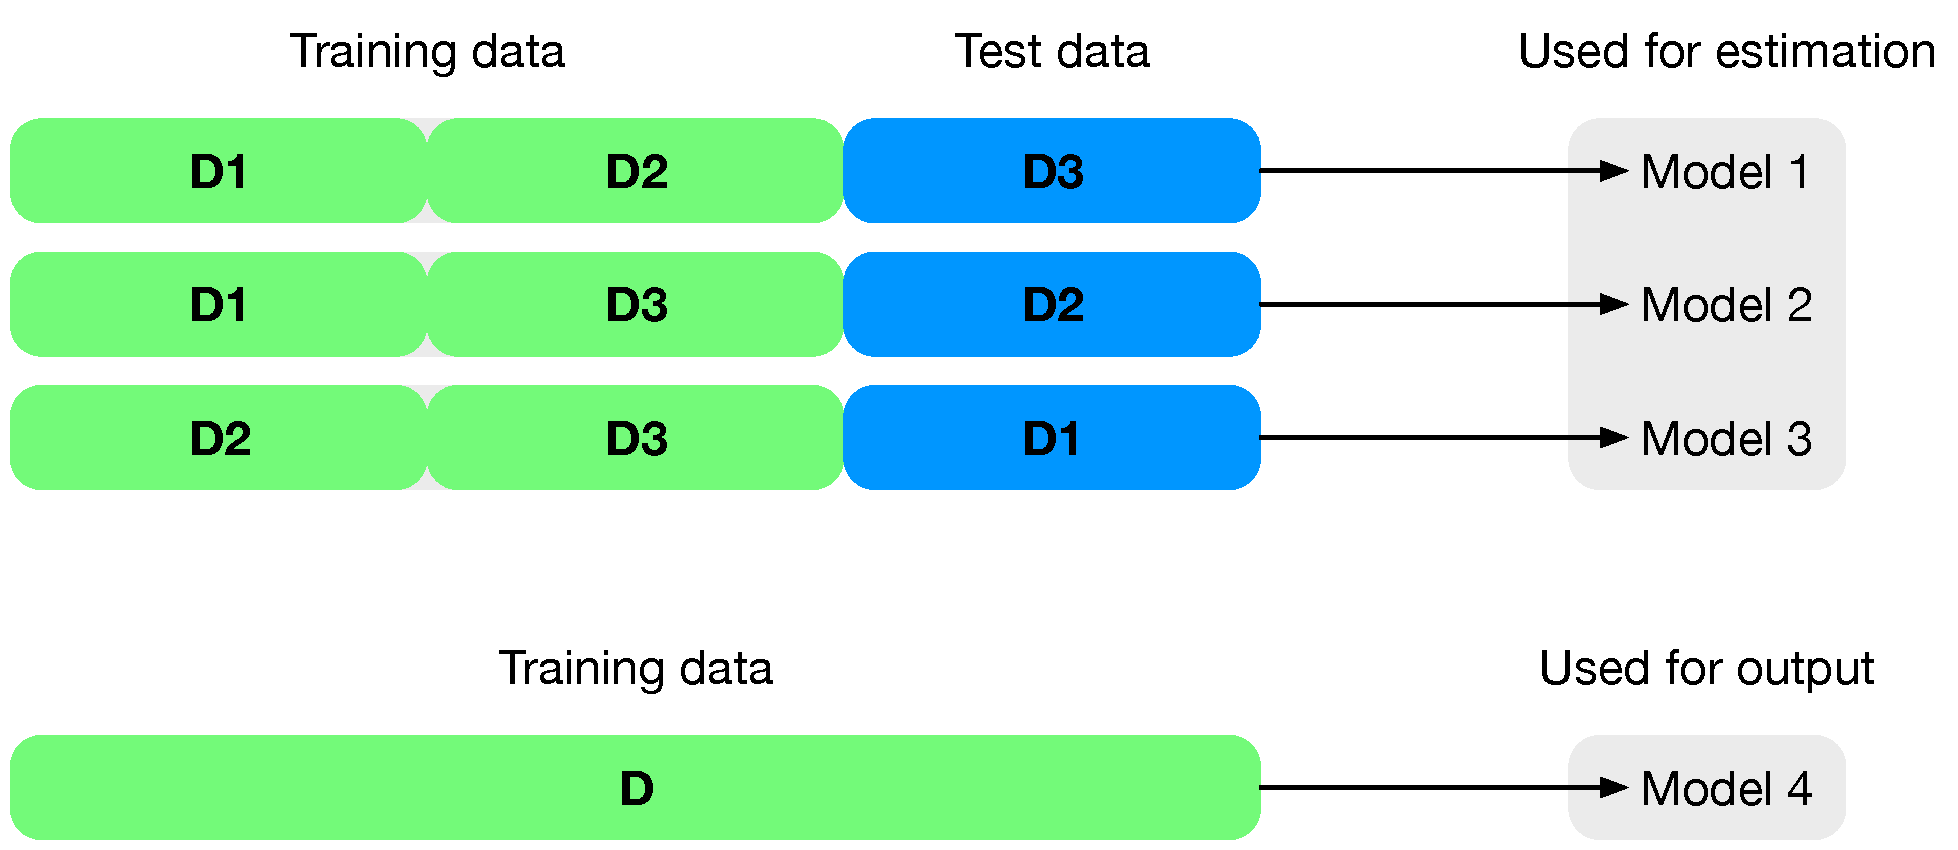
\includegraphics[width=0.9\textwidth]{plots/cv/cv-workflows-retrain}
   \label{fig:workflow0}
   \caption{Model 1, 2, and 3 are used only for performance estimation and are then thrown away. A final model (model 4) is trained using the complete dataset.}
\end{center}
\end{figure}

\paragraph{Cross validation in application}
A problem with the previous approach is that the estimation is not done for the final model, but rather of the average final model. This complicates statistical uncertainty analysis.

One approach to get the benefits of the extended test set, while estimating the performance of the final model is to assign to each event a unique identifier. Fold assignment is then done by evaluating a deterministic expression with the identifier as input.

This approach is sometimes called cross evaluation and allows us to use all K models generated by the k-folds cross validation procedure in application. 

\begin{figure}
\begin{center}
   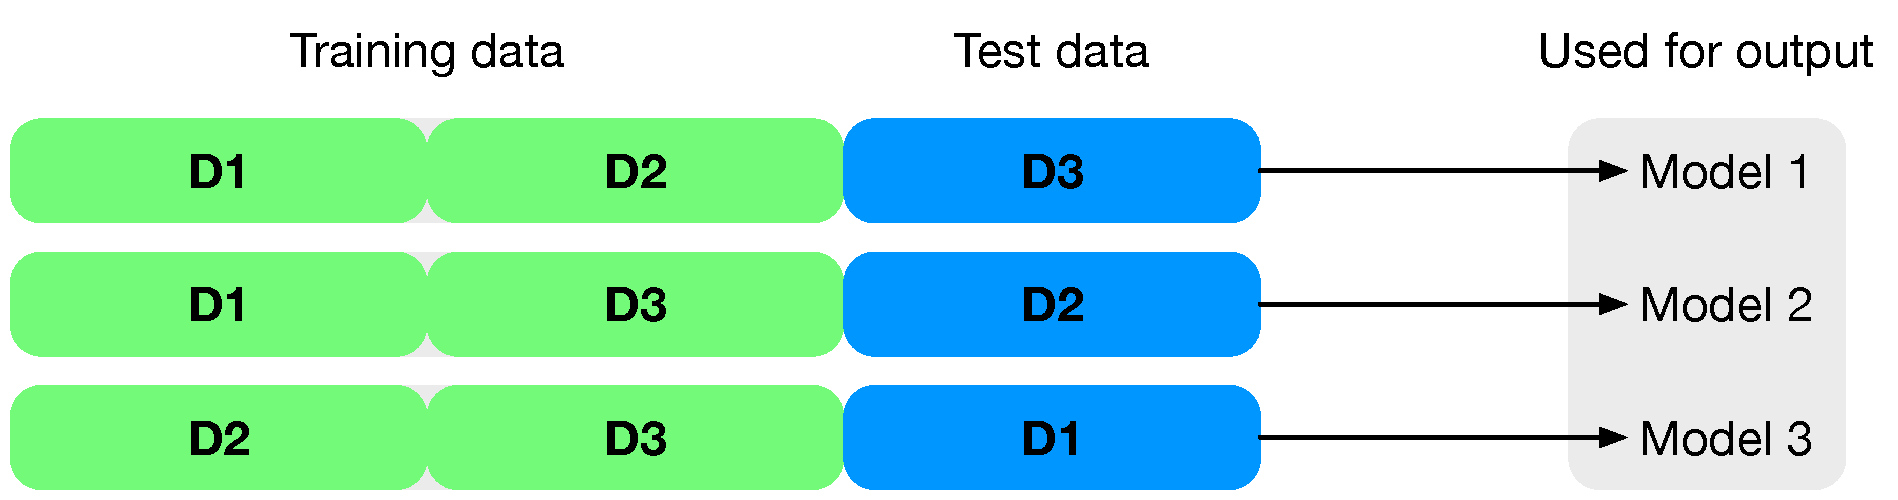
\includegraphics[width=0.9\textwidth]{plots/cv/cv-workflows-ce}
   \label{fig:workflow1}
   \caption{Model 1, 2, and 3 are used for performance estimation and as the final output model. This is made possible by the introduction of the split expression which assigns each processed event to a unique model.}
\end{center}
\end{figure}











% ============================================================================
% === Implementation
% ============================================================================
\subsubsection{Implementation}

% Features
% - Supports classification, multiclass, regression
% - Supports k-folds crossvalidation with random split, and by evaluating an expression
% - Supports simplified access to results, and offline analysis with TMVA Gui (all three analysis types)
% - Support application to data through 2 schemes, described above


Cross validation in TMVA is implemented as a wrapper around the Factory class. This means the cross validated work flow uses a separate entry point, but effort is made to maintain similarity between the two interfaces. Do note however that there is a difference in how the dataloader is handled. For the Factory a separate dataloader can be associated with each booked method, in cross validation the same dataloader is applied to all booked methods. See Example~\ref{code:cv-minimal} for an example of a simple set up.

Cross validation is supported for all analysis types that the Factory supports, i.e. Classification, Regression and Multiclass.

After training and evaluation, output files suitable for analysis with the different TMVA GUIs can be generated. All analysis types are supported with some caveats.

The current cross validation implementation supports k-folds splitting. This splitting mechanism is implemented separately from the dataset splitting mechanism and currently only uses events the dataloader puts in the test set. See Example~\ref{code:cv-dataloader} for an example of how this is done for a simple Classification set up.

The k-folds splitting mechanism supports two modes of operations. Random splitting and functional splitting. The random splitting is activated when the splitExpr option is left out or given as the empty string. In this case events are assigned to folds randomly (where the random generator is seeded with the seed provided in the option SplitSeed). Random splitting is only supported for training and evaluation, not in the application phase. This makes it suitable for quickly getting up and running, trying different methods out, but not for final analysis and application to data.
% Performance estimation using method 1 or PE + application as in method 2.

For data application, the second mode of operation, functional splitting, is preferred. Using the option splitExpr you can define an expression that is evaluated for each event. The result of evaluation is used for fold assignment. See Section~\ref{sec:k-folds-splitting} for more details.

\begin{codeexample}
\begin{tmvacode}
auto d = new TMVA::DataLoader("<datasetName");
d->AddVariable("x");
d->AddSpectator("eventID");
d->AddSignalTree(sigTree);
d->AddBackgroundTree(bkgTree);
d->PrepareTrainingAndTestTree("", "nTest_Signal=0"
                                  ":nTest_Background=0");
\end{tmvacode}
\caption[.]{\codeexampleCaptionSize
Setting up a typical dataloader for using with cross validation. It is assumed that you have available to TTrees, one with signal events, one with background events, both with suitable variables defined.
Cross validation in TMVA uses a separate splitting mechanism which is applied after the ordinary splitting step. It uses only events in the training set, the test set is currently left unused. To make all events available to cross validation, they are placed in the training set by setting the size of the test set to zero.
}
\label{code:cv-dataloader}
\end{codeexample}

\begin{codeexample}
\begin{tmvacode}
auto d = new TMVA::DataLoader("<datasetName>");
auto f = TFile::Open("path/to/file");
TString opt = "!V:!Silent:!Correlations"
              ":AnalysisType=Classification"
              ":NumFolds=2";
TMVA::CrossValidation cv {"<jobname>", d, f, opt};

cv.BookMethod(TMVA::Types::kBDT, "BDT", "<options>");
cv.Evaluate();
\end{tmvacode}
\caption[.]{\codeexampleCaptionSize Minimal example to get cross validation up and running using the dataloader defined in \ref{code:cv-dataloader}. The example sets up a cross validated BDT with 2 folds where the folds are assigned randomly. The results will be available for inspection with the TMVA GUI interface under \texttt{"path/to/file"}.}
\label{code:cv-minimal}
\end{codeexample}











% ============================================================================
% === Options
% ============================================================================
\subsubsection{Cross validation options}

Constructing a \texttt{CrossValidation} object is very similar to how one would construct a TMVA Factory with the exception of how the data loader is handled. In TMVA cross validation, you are responsible for constructing the data loader. When passed to the \texttt{CrossValidation} constructor it takes ownership and makes sure that the memory is properly released after training and evaluation.

An schematic of how to construct a new \texttt{CrossValidation} object is detailed in Code Example~\ref{code:cv-constructor}.

\begin{codeexample}
\begin{tmvacode}
CrossValidation cv {"<jobname>", dataloader, "<options>"};
\end{tmvacode}
\caption[.]{\codeexampleCaptionSize Constructing a CrossValidation instance:
   the first argument is a job name, which will get prepended to all files
   produced by the CrossValidation factory; The second is the data loader that
   will provide data for all methods booked through the CrossValidation class;
   The third is a list of options configuring this instance. Available options
   can be found in Table~\ref{tab:cv:options}.
   Individual options are separated by a ':'. See
   Sec.~\ref{sec:usingtmva:booking} for more information on the booking.}
\label{code:cv-constructor}
\end{codeexample}

\texttt{CrossValidation} wraps a TMVA Factory internally and thus supports all options that the Factory supports. In addition it, can be configured with the following options.

\begin{optiontableAuto}
SplitExpr & \mc{1}{c}{--} &  &  \mc{1}{l}{--} 
          & Expression used to assign events to folds. If not given or given as "" events will be assigned to folds randomly. \\

SplitSeed & \mc{1}{c}{--} & 0 &  \mc{1}{l}{--} 
          & Only used when SplitExpr is "". Determines the seed for the random assignment of events to folds. \\

NumFolds & \mc{1}{c}{--} & 2 &  \mc{1}{l}{--} 
         & Number of folds to generate. \\

FoldFileOutput & \mc{1}{c}{--} & False &  \mc{1}{l}{--} 
         & If given a TMVA output file will be generated for each fold.
           File name will be the same as specified for the combined output with
           a \_foldX suffix. \\

OutputEnsembling & \mc{1}{c}{--} & "None" & "None", "Avg"
         & Combines output from contained methods (only in application phase).
           If None, SplitExpr is used to assign event to fold, no combination
           is performed. Valid values are "None", and "Avg". \\
\end{optiontableAuto}











% ============================================================================
% === K-folds
% ============================================================================
\subsubsection{K-folds splitting}
\label{sec:k-folds-splitting}
TMVA currently supports k-folds cross validation. In this scheme, events are assigned to one of $K$ folds. The training is then run $K$ times, each time using one fold as the test data and the rest as training data. TMVA supports to modes of assigning events to folds: Random assignment, and assignment through an expression. The option \texttt{SplitExpr} selects what mode to use and what expression to evaluate.

The splitting mechanism used by the k-folds implementation is different from the one that the TMVA dataloader uses to partition the input into a training and test set. With k-folds, only events in the training set after \texttt{PrepareTrainingAndTestTree} has been called are picked up by the k-folds splitting. To use all available events for cross validation one can explicitly set the number of test events to zero, as is shown in Code Example~\ref{code:cv-prepare-dataset}.

\begin{codeexample}
\begin{tmvacode}
dataloader.PrepareTrainingAndTestTree("<sigcut>", "<bkgcut>",
   "<options>:nTest_Signal=0:nTest_Background=0");
\end{tmvacode}
\caption[.]{\codeexampleCaptionSize }
\label{code:cv-prepare-dataset}
\end{codeexample}

\paragraph{Random splitting}
Random splitting is the default mode of operation if \texttt{SplitExpr} is not specified to the \texttt{CrossValidation} constructor, or if it is given as \texttt{"SplitExpr="}.

Random splitting is usually used to estimate the performance of a training scheme. After the estimation a final model is created by retraining the method on all available training data. This final model is then applied to new, unlabelled data. More details can be found in \ref{sec:cv-performace-estimation-methods}.

Be careful if using the resulting models in the TMVA application phase and ensure that you use a separate dataset that has not been used for training. Since the training error can be significantly smaller than the generalisation error, there estimate thus derived will be optimistically biased. This applies equally to a model trained on the complete data set as well as the models resulting from the individual folds.

\paragraph{Splitting with an expression}
If an expression is provided to the \texttt{CrossValidation} constructor through the option \texttt{SplitExpr}, events will be assigned to folds according to this expression. This is true both for training and application.

The expression can use spectators defined in the dataset and a special variable \texttt{numFolds} that will be replaced with the corresponding concrete number at split time.

The idea behind using an expression for splitting is to generate a final model for which the performance estimates acquired through cross validation applies. As such the result of evaluating the expression should in essence be a uniformly distributed random number, independent of the content of an event. It is therefore preferred to assign a globally unique number to event at creation time and use this as input. 

An example can be seen in Code Example~\ref{code:cv-split-expr}. The syntax is a consequence of the expression being backed by a TFormula. Spectators and context variables are made available through \texttt{TFormula} named parameters, which are accessed with brackets \texttt{"[]"}. \texttt{TFormula}s only handle floating point operands which necessitates the integer casts. See the documentation of \texttt{TFormula} for more information on syntax.

\begin{codeexample}
\begin{tmvacode}
auto * d = new TMVA::DataLoader("<name>");
d.AddVariable("x");
d.AddVariable("y");
d.AddSpectator("eventNumber");

TString splitExpr = "int([eventNumber])\%int([numFolds])";
TString options = TString::Format("SplitExpr=\%s", splitExpr);

TMVA::CrossValidation cv {"<jobname>", d, options};
\end{tmvacode}
\caption[.]{\codeexampleCaptionSize The split expression uses spectators defined on the \texttt{TMVA::DataSet} to calculate the fold assignment for each fold. Note that code for adding data, methods, and for training has been abbreviated.
}
\label{code:cv-split-expr}
\end{codeexample}










% ============================================================================
% === Output
% ============================================================================
\subsubsection{Output}
\label{sec:cv-output}
Cross validation in TMVA provides several different outputs to facilitate analysis. Firstly, a file suitable for analysis with the guis presented in Section~\ref{sec:displayingResults} is produced after a successful training.

One can also request the generation of additional files for per-fold analysis with the guis.

Finally, a selection of statistics are collected during training and made available through a programmatic interface.

\paragraph{Offline analysis through the TMVA Gui}
\label{sec:cv-output-files}
% Analysis with TMVA Gui

Output files suitable for analysis with the TMVA Gui is produced after a completed training if a \texttt{TFile} is provided the \texttt{CrossValidation} constructor. For each fold, the independent test set is evaluated and added to the output file.

Optionally files with \emph{per-fold} training and test set output files can be generated. 

All analysis types are supported, i.e. classification, multiclass, and regression.

The provided output file will be contain all events provided the test set, since k-folds splitting can ensure that each training event belongs only to one test set.

Do note that the training set produced when using the TMVA Factory is difficult to define in a meaningful way here since each event will be used as training, multiple times, and test event. However, for implementation considerations the training set will still be present in the output file. 

In the current version it is a copy of the test set, however the contents of the training set cannot be depended on as it may change in future releases.

To generate output files for offline analysis of the separate folds one submits the option \texttt{foldOutputFiles=True} to the \texttt{CrossValidation} constructor. The output files will use the same name as the provided \texttt{TFile}, with an extra suffix, \texttt{\_foldK}, where $K$ indicates the corresponding fold.

There are no caveats when analysing the \emph{per-fold} output files, as compared to above.

\begin{codeexample}
\begin{tmvacode}
root -l -e 'TMVA::TMVAGui("<path/to/file>")'
\end{tmvacode}
\caption[.]{\codeexampleCaptionSize Command line command to run to inspect the resulting output file using the classification GUI.
For the multiclass and regression GUIs, use \texttt{TMVA::TMVAMultiClassGui} and \texttt{TMVA::TMVARegressionGui} respectively. Note that \texttt{"<path/to/file>"} can be either the output file provided to the \texttt{CrossValidation} constructor, or one of the fold outputs.
The per-fold output files have the same name, with an extra suffix, \texttt{\_foldK}, where $K$ indicates fold id.}
\label{code:cv-gui}
\end{codeexample}

\paragraph{Summary statistics after training}
\label{sec:cv-output-prog}

Some statistics are collected during training and evaluation on a per-fold basis. These are made available through the \texttt{TMVA::CrossValidation::GetResults} method.

Tracked metrics include, ROC curves and integral, signal significance, separation and background efficiencies.

An example of how this is used in practise is seen in Code Example~\ref{code:cv-results} and an example output of running that code can be seen in Code Example~\ref{code:cv-results-output}.

For full documentation of available statistics, see \url{root.cern.ch/doc/master/classTMVA_1_1CrossValidationResult.html}.

\begin{codeexample}
\begin{tmvacode}
TMVA::CrossValidation cv {"<jobname>", <dataloader>, <outputFile>, "<options>"};
cv.BookMethod(<methodType>, "<methodName>", "<options>");
cv.Evaluate();

size_t iMethod = 0;
for (auto && result : cv.GetResults()) {
   std::cout << "Summary for method "
             << cv.GetMethods()[iMethod++].GetValue<TString>("MethodName")
             << std::endl;
   for (UInt_t iFold = 0; iFold<cv.GetNumFolds(); ++iFold) {
      std::cout << "\tFold " << iFold << ": "
                << "ROC int: " << result.GetROCValues()[iFold]
                << ", "
                << "BkgEff@SigEff=0.3: " << result.GetEff30Values()[iFold]
                << std::endl;
   }
}
\end{tmvacode}
\caption[.]{\codeexampleCaptionSize Statistics is available through the CrossValidationResults object. For example, ROC integrals and efficiencies can be accessed per fold. See the ROOT reference for up to date interface documentation.}
\label{code:cv-results}
\end{codeexample}

\begin{codeexample}
\begin{tmvacode}
Summary for method BDT
   Fold 0: ROC int: 0.961109, BkgEff@SigEff=0.3: 0.961
   Fold 1: ROC int: 0.974712, BkgEff@SigEff=0.3: 0.986
Summary for method Fisher
   Fold 0: ROC int: 0.964606, BkgEff@SigEff=0.3: 0.963
   Fold 1: ROC int: 0.977215, BkgEff@SigEff=0.3: 0.992
\end{tmvacode}
\caption[.]{\codeexampleCaptionSize Example output when running the code in Code Example~\ref{code:cv-results}.}
\label{code:cv-results-output}
\end{codeexample}

% See documentation for CrossValidationResults











% ============================================================================
% === Application
% ============================================================================
\subsubsection{Application}
\label{sec:cv-application}

Application is the phase where the model is presented with new, unlabelled data. This requires a final model which is ready to accept events. The naive approach of cross validation does not produce a final model to be evaluated, but instead produces one model for each fold. Generating a such a model can be done in a multitude of ways including the approaches presented in Section~\ref{sec:cv-workflows}.

When using the first approach, retraining your model on the complete data set, you would do this using the TMVA Factory as detailed in Section~\ref{sec:usingtmva:factory} and the process of applying data using the TMVA Reader as detailed in section~\ref{sec:usingtmva:reader}.

When using the second approach, cross validation in application, TMVA simplifies the process for you. You need to specify a split expression so that TMVA can partition the input data. After training, a combined model is produced, containing the models for the folds and the split expression.

This model can be used with the regular TMVA Reader and ensures that applied events are evaluated by the corresponding model, as indicated by the split expression. You as the end-user need only ensure that the same variables and spectators are defined for the application data set as in training, and that the weight files for each fold model reside in the same directory as the combined model.

\begin{codeexample}
\begin{tmvacode}
TMVA::Reader reader {"!Color:!Silent:!V"};

reader.AddVariable("x", &x);
reader.AddVariable("y", &y);
reader.AddSpectator("eventID", &eventID);

reader.BookMVA("<methodName>", "<path/to/weight/file.xml>");
\end{tmvacode}
\caption[.]{\codeexampleCaptionSize Using a model training with cross validation in application uses the same interface as the non cross validated case. One must make sure, however, that the variable and spectator declarations are the same as in training, and the per-fold model weight files reside in the same folder as the combined model weight file specified by \texttt{"<path/to/weight/file.xml>"}.}
\label{code:cv-application}
\end{codeexample}
